\section{Menu Phase: 2D Renderer}
The menu phase is renderer by the 2D renderer which is tile based. The screen is divided into tiles as follow:\\
DRAWING\\
Bla bla bla\\
Assets are called "pic" as opposed to sprites in 3D phases. Pics  are all Huffman-compressed (VGADICT, VGAHEAD, 
VGAGRAPH).

 \begin{figure}[H]
\centering
 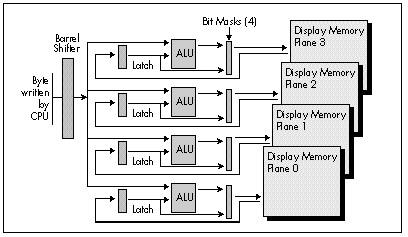
\includegraphics[width=\textwidth]{imgs/latches_drawing.png}
 \end{figure}

Not at fast as it seems since things have to be drawn in all three buffers during action 3D phase:\\
\par

\begin{minipage}{\textwidth}
\lstinputlisting[language=C]{code/StatusDrawPic.c}
\end{minipage}


LatchDrawPic
Chapter 48 from michael abrash book
atches were not intended for use in 256-color mode; that was something I figured out as a hack and wrote about. The latches were used so that in 16-color mode any or all of the four planes could be written to at once.
\par
\begin{figure}[H]
\centering
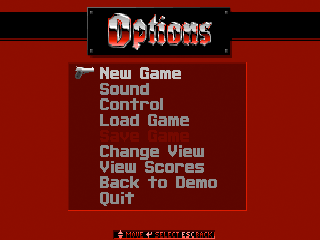
\includegraphics[width=\textwidth]{imgs/first_menu.png}
\caption{Architecture and sub-systems.}
\end{figure}